\documentclass[a4paper]{article}
\usepackage{amsmath,amssymb,booktabs,caption,float,graphicx,xcolor}
\usepackage{minted}
\usepackage[utf8]{inputenc}
\usepackage[english]{babel}
\usepackage[backend=bibtex]{biblatex}
\addbibresource{Homework7.bib}
% \captionsetup[figure]{labelsep=period}
\captionsetup[table]{labelsep=period}
\definecolor{bg}{rgb}{0.95,0.95,0.95}
\renewcommand\thesection{\arabic{section}}
\usemintedstyle{emacs}
\begin{document}
\begin{center}
    \huge
    \textbf{VE482\\Introduction to Operating Systems\\}
    \Large
    \vspace{15pt}
    \uppercase{\textbf{Homework 7}}\\
    \large
    \vspace{5pt}\today\\
    \vspace{5pt}
    Yihua Liu 518021910998
    \vspace{5pt}
    \rule[-5pt]{.97\linewidth}{0.05em}
\end{center}
\section*{Ex. 1 — Page replacement algorithm}
\begin{enumerate}
    \item Explain the content of the new table entries if a clock interrupt occurs at tick 10.\\
    If a clock interrupt occurs at tick 10, the referenced bits will be cleared:
    \begin{table}[H]
        \centering
        \begin{tabular}{ccccc}
            \toprule
            Page&Time stamp&Present&Referenced&Modified\\
            \midrule
            0&6&1&0&1\\
            1&9&1&0&0\\
            2&9&1&0&1\\
            3&7&1&0&0\\
            4&4&0&0&0\\
            \bottomrule
        \end{tabular}
        \caption{The system state when a clock interrupt occurs at tick 10.}
    \end{table}
    \item Due to a read request to page 4 a page fault occurs at tick 10. Describe the new table entry.\\
    Suppose the scheduled write is not completed, the new table entries are:
    \begin{table}[H]
        \centering
        \begin{tabular}{ccccc}
            \toprule
            Page&Time stamp&Present&Referenced&Modified\\
            \midrule
            0&6&1&0&1\\
            1&9&1&0&0\\
            2&9&1&0&1\\
            3&10&1&1&0\\
            4&4&0&0&0\\
            \bottomrule
        \end{tabular}
        \caption{The new table entries.}
    \end{table}
\end{enumerate}
\section*{Ex. 2 — Minix 3}
The goal of this exercise is to understand and implement system calls.
\begin{enumerate}
    \item In which files are:
    \begin{enumerate}
        \item the constants with number and name for the system calls?\\
        In \texttt{/usr/src/include/minix/callnr.h}
        \item the names of the system call routines?\\
        In \texttt{/usr/src/servers/pm/table.c}
        \item the prototypes of the system call routines?\\
        In \texttt{/usr/src/servers/pm/proto.h}
        \item the system calls of type “signal” coded?\\
        In \texttt{/usr/src/servers/pm/signal.c}
    \end{enumerate}
    \item What problems arise when trying to implement a system call \texttt{int getchpids(int n, pid\_t *childpid)} which “writes” the pids of up to $n$ children of the current process into \texttt{*childpid}?\\
    % System calls are the interface between the kernel space and user space. If this system call is implemented, users can use this system call to control the process IDs as they want, which is very dangerous, because there might be conflicts. Process IDs are managed by the operating system.
    The order of the printed process identifiers of children processes might be un-determined.
    \item Write a “sub-system call” \texttt{int getnchpid(int n, pid\_t childpid)} which retrieves the $n$-th child process.\\
    At the end of \texttt{/usr/src/servers/pm/utility.c},
    \begin{minted}[frame=single,bgcolor=bg,breaklines,breakanywhere,linenos]{c}
/*===========================================================================*
 *			      do_getnchpid                                   *
 *===========================================================================*/
 int do_getnchpid(int n, pid_t *p_children)
{
  register struct mproc *rmp;
  
  if (p_children == NULL || n > NR_PROCS)
  	return EINVAL;
  rmp = &mproc[n];
  if (rmp->mp_parent != who_p)
  	return EBADSRCDST;
  *p_children = rmp->mp_pid;
  return OK;
}
    \end{minted}
    \item Using the previous sub-system call, implement the original \texttt{getchpids} system call. The returned int value corresponds to the number of pids in \texttt{*childpid}, or -1 on an error.
    At the end of \texttt{/usr/src/servers/pm/utility.c},
    \begin{minted}[frame=single,bgcolor=bg,breaklines,breakanywhere,linenos]{c}
/*============================================================================*
 *                            do_getchpids                                    *
 *============================================================================*/
 int do_getchpids(int n, pid_t *p_children)
{
  int i;
  
  for (i = 0; i < n; i++) {
    if (do_getnchpid(i, p_children + i) != OK) {
      i = -1;
      break;
    }
  }
  
  return i;
}
    \end{minted}
    At Line 57 of \texttt{/usr/src/include/minix/callnr.h}, add
    \begin{minted}[frame=single,bgcolor=bg,breaklines]{c}
#define GETCHPIDS	  56
    \end{minted}
    Change Line 70 of \texttt{/usr/src/servers/pm/table.c} into
    \begin{minted}[frame=single,bgcolor=bg,breaklines]{c}
	do_getchpids,	/* 56 = getchpids */
    \end{minted}
    At the end of \texttt{/usr/src/servers/pm/proto.h}, add
    \begin{minted}[frame=single,bgcolor=bg,breaklines]{c}
int do_getnchpid(int n, pid_t *p_children);
int do_getchpids(int n, pid_t *p_children);
    \end{minted}
    \item Write a short program that demonstrate the previous system calls.
    \begin{minted}[frame=single,bgcolor=bg,breaklines]{c}
#include <unistd.h>
#include <stdio.h>

#define CHILD_NUM 10

int main() {
  int i, n_children = 0;
  pid_t p_children[CHILD_NUM], p_children_std[CHILD_NUM];

  while (n_children <= CHILD_NUM / 2) {
    pid_t pid = fork();
    if (pid == 0)
      p_children_std[n_children++] = pid;
    else
      exit(0);
  }
  
  getchpid(n_children, p_children);
  
  for (i = 0; i < n_children; i++) {
    if (p_children_std[i] != p_children[i]) {
      fprintf(stderr, "Wrong answer %d\n", i);
    }
  }

  return 0;
}
    \end{minted}
    \item The above strategy solves the initial problem through the introduction of a sub-system call.
    \begin{enumerate}
        \item What are the drawbacks and benefits of this solution?\\
        Drawbacks: it is not efficient to traverse all the processes.\\
        Benefits: it is flexible because it can be used by other system calls; it is easy to implement.
        \item Can you think of any alternative approach? If yes, provide basic details, without any implementation.\\
        Use a tree to traverse the parent and child processes to improve efficiency.
    \end{enumerate}
\end{enumerate}
\section*{Ex. 3 — Research}
Write about a page on the topic of the \texttt{ext2} filesystem. Do not forget to reference your sources.
\begin{figure}[H]
    \centering
    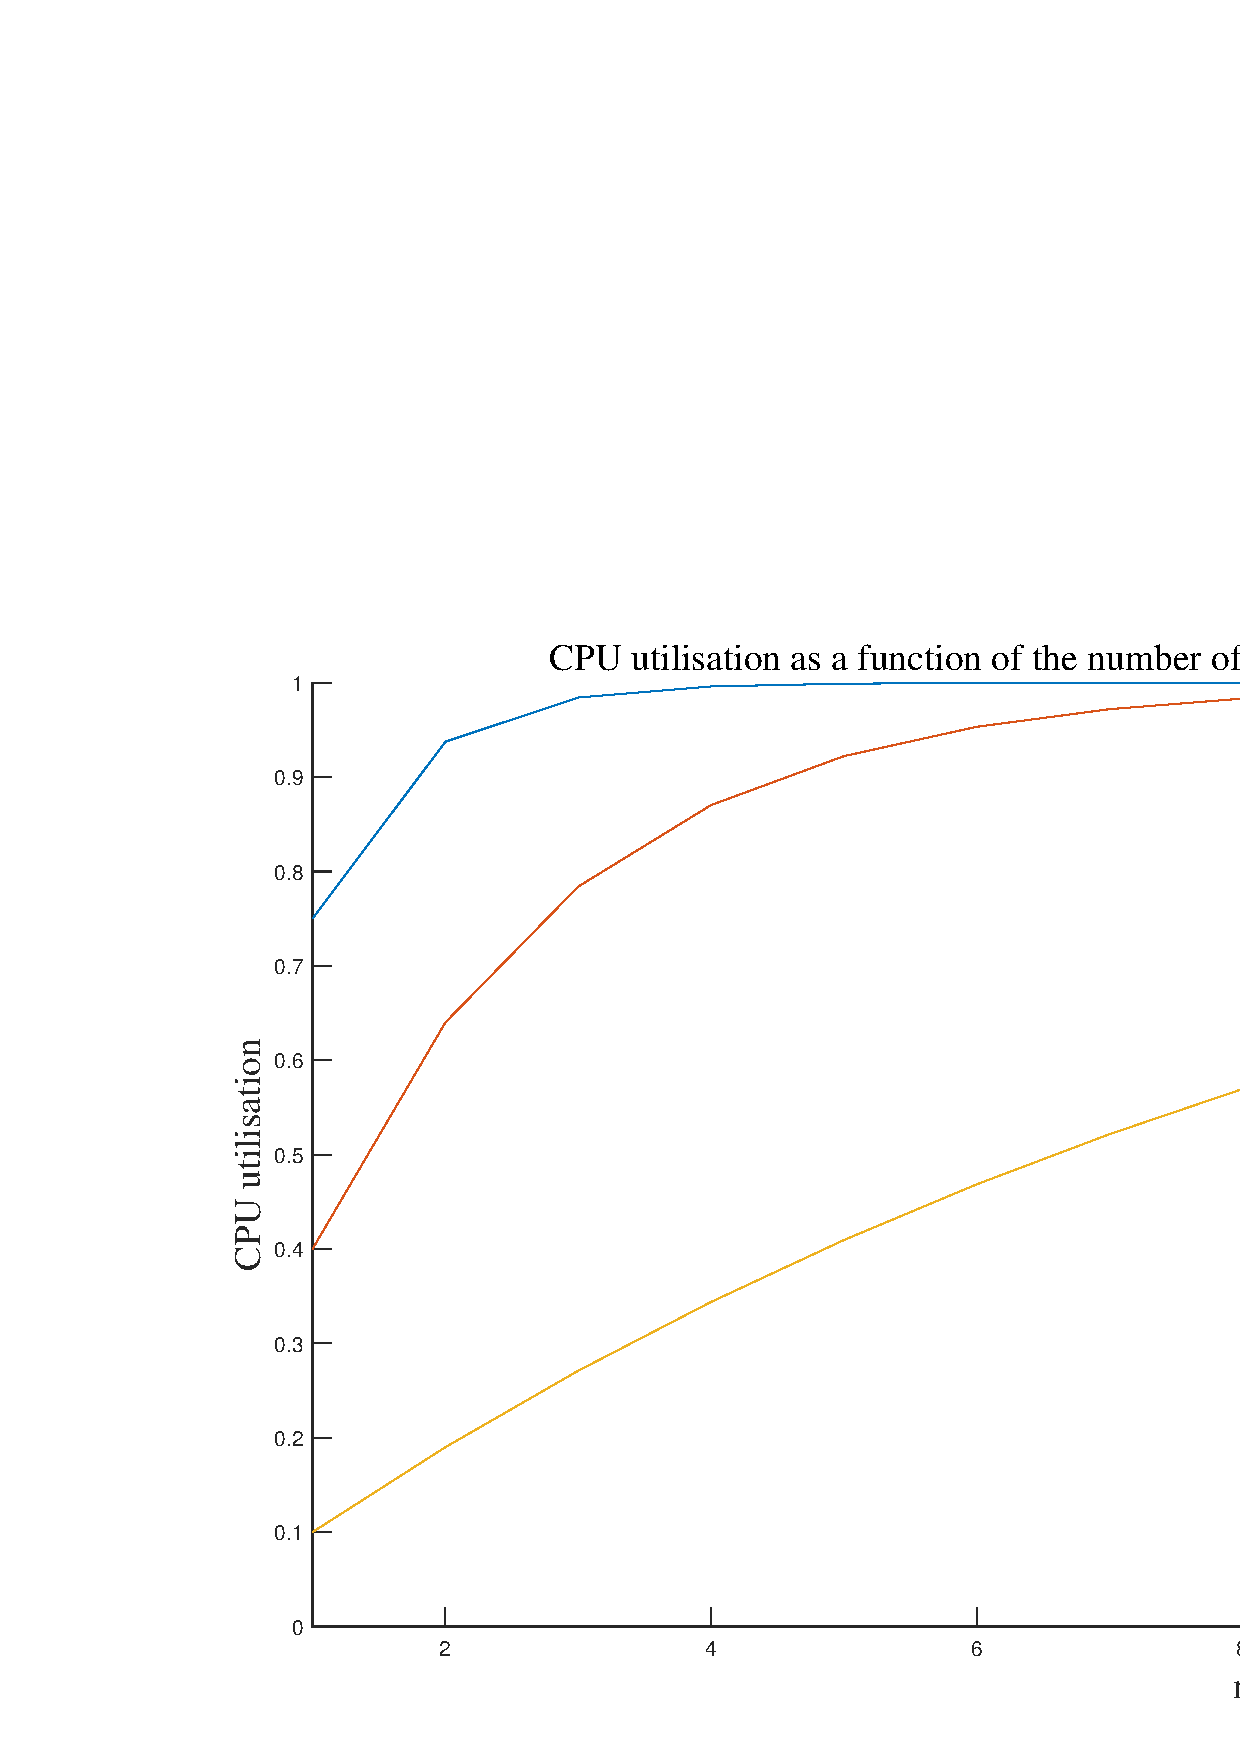
\includegraphics[width=1\textwidth]{1.png}
    \caption{Physical Layout of the EXT2 File system \cite{science}.}
\end{figure}
\texttt{ext2} is a file system for the Linux kernel. Its full name is second extended file system. It was invented by Rémy Card, Theodore Ts'o and Stephen Tweedie. It is also adopted by other systems like Microsoft Windows, MacOS, and Minix 3.

The basic structure of \texttt{ext2} is blocks. "A partition, disk, file or block device" formatted with a "Second Extended Filesystem is divided into small groups of sectors called 'blocks'" \cite{nongnu}.

Many blocks construct block groups, which contains copies of superblocks and block group descriptor tables, and the group descriptor stores "the location of the block bitmap, inode bitmap, and the start of the inode table for every block group" \cite{ext2wiki}. The block groups used to "reduce fragmentation" and minimize "the amount of head seeking when reading a large amount of consecutive data" \cite{kerneldoc}.

In details, The EXT2 group descriptor is the data structure describing the block group that contains blocks bitmap, inode bitmap, inode table, free blocks count, free inodes count, and used directory count \cite{science}.
\begin{figure}[H]
    \centering
    \includegraphics[width=1\textwidth]{2.png}
    \caption{The EXT2 Inode \cite{science}.}
\end{figure}
The superblock, containing the configuration of the file system like the total number of inodes and blocks, are stored on disks in the format of little endian. Here inodes (whose full name is index node) are representations of files or directories.

The data structure of inodes stores the "the size, permission, ownership, and location on disk of the file or directory" \cite{ext2wiki}. In detail, inodes contains mode, owner information, size, timestamps, and datablocks.

Directories are all like a file with an inode but also associates file names and inode numbers.

In detail, a directory is a linked list data structure. Every linked list contains "the name of the entry, the inode associated with the data of this entry, and the distance within the directory file to the next entry" \cite{nongnu}.
\begin{table}[H]
    \centering
    \begin{tabular}{|c|c|}
        \hline
        Block size&Maximum file size\\
        \hline
        1024&16 GiB\\
        \hline
        2048&256 GiB\\
        \hline
        4096&2 TiB\\
        \hline
    \end{tabular}
    \caption{Block and file sizes in the second extended filesystem \cite{proflinuxk}.}
\end{table}
\section*{Ex. 4 — Simple questions}
\begin{enumerate}
    \item If a page is shared between two processes, is it possible that the page is read-only for one process and read-write for the other? Why or why not?\\
    ‌No, it is not. Because the process with read-write permission to the shared page makes a copy of that page when updating that page, thus there will be two page copies. The page is no longer shared between the two process.
    \item A computer provides each process with 65,536 bytes of address space divided into pages of 4096 bytes. A particular program has a text size of 32,768 bytes, a data size of 16,386 bytes, and a stack size of 15,870 bytes. Will this program fit in the address space? If the page size were 512 bytes, would it fit?\\
    If the page size were 4096 bytes, it would not fit.\\
    If the page size were 512 bytes, it would fit.
    \item When both paging and segmentation are being used, first the segment descriptor is found and then the page descriptor. Does the TLB also need a two-levels lookup?\\
    It depends. If the page table is small, one-level TLB is small and fast enough. However, if the page table is huge and we want higher performance, two-level TLB can be introduced. A small level 1 TLB is extremely fast and small while a larger level 2 TLB is relatively slower.
\end{enumerate}
\printbibliography
\end{document}